\section{Introduzione}

\subsection{Funzionamento}\label{sec:intro}
ABP (\emph{Alternating Bit Protocol}) è un protocollo di rete operante al
livello data link.

Tale tecnologia si assicura che la comunicazione tra due nodi adiacenti avvenga
correttamente, adottando le seguenti regole:

\begin{itemize}
  \item I messaggi vengono spediti unidirezionalmente, dal
    trasmittente A (o \emph{Sender}) al ricevente B (o
    \emph{Receiver})\footnote{si assume che il canale di trasmissione sia di
    tipo FIFO};
  \item Ad ogni messaggio è abbinato un numero (un bit) che indica il numero di
    sequenza, 0 o 1;
  \item Ogni messaggio che A deve trasmettere ha numero di sequenza diverso dal
    messaggio successivo che deve spedire;
  \item Alla ricezione del messaggio, B può mandare ad A:
  \begin{itemize}
    \item un messaggio di conferma di corretta ricezione
      (\emph{Acknowledgement}) \texttt{ACKX}, dove X è il numero di sequenza
      del messaggio ricevuto;
    \item un messaggio di conferma di ricezione con errori
      (\emph{Negative Acknowledgement}) \texttt{NACKX}, dove X è il numero di
      sequenza del messaggio ricevuto.
  \end{itemize}
  \item I messaggi vengono trasmessi continuamente da A senza rimanere
    bloccato in attesa di una qualsiasi risposta da B;
  \item Nel caso in cui A ricevesse un \emph{acknowledgement} per il messaggio
    che sta trasmettendo, deve cominciare la trasmissione del prossimo
    messaggio;
  \item finchè A sta trasmettendo un messaggio con numero di sequenza, tutti
    gli \texttt{ACK} e i \texttt{NACK} con numero di sequenza diverso dovranno
    essere ignorati.
\end{itemize}

\begin{figure}[H]
  \centering
  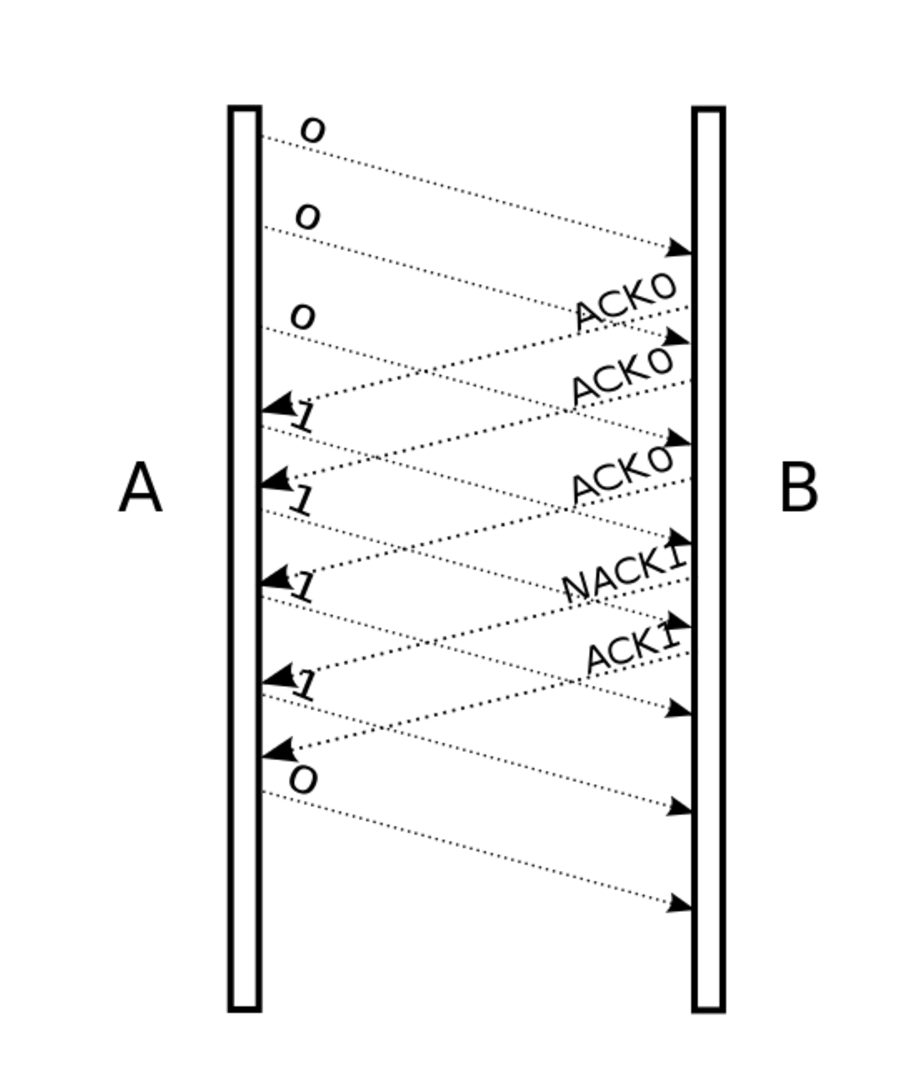
\includegraphics[width=.5\columnwidth]{images/abp.eps}
  \caption{Protocollo ABP}
  \label{fig:graphic-abp}
\end{figure}
